% !TEX encoding = UTF-8
% !TEX TS-program = pdflatex
% !TEX root = ../tesi.tex

%**************************************************************
\chapter{Introduction}\label{ch:introduction}
%**************************************************************

\intro{In this section will be summarized the content of the whole thesis.}
%\noindent Esempio di utilizzo di un termine nel glossario \\
%\gls{api}. \\
%
%\noindent Esempio di citazione in linea \\
%\cite{site:agile-manifesto}. \\
%
%\noindent Esempio di citazione nel pie' di pagina \\
%citazione\footcite{womak:lean-thinking} \\


\section{Background}\label{sec:background}

In recent years, the field of computer vision has been growing in complexity and the number of applications has been increasing, main applications are: image classification, object detection, face recognition, image segmentation, \gls{slam} and visual odometry which is a task in which the robot is able to understand where it is and how it is oriented.

The development of computer vision has been a long process, the growth is favoured by the development of new hardware components and new challenges, about the latters, we have
CIFAR-10 (Doon et al.~\cite{cifar10_paper}), Fashion-MNIST(Xiao et al.~\cite{fashion_mnist_paper}), MS-Coco (Lin et al.~\cite{ms_coco_paper}) and ImageNet (Deng et al.~\cite{imagenet_paper}).
These datasets are often used as benchmark for novel models.

For the architectures, starting from AlexNet (Krizhevsky et al.~\cite{alex_net_paper}), then VGG (Simonyan et al.~\cite{vgg_paper}), Inception-V1 (Szegedy et al.~\cite{inception_v1_paper}), Inception-V2(Szegedy et al.~\cite{inception_v2_paper}), ResNet (He et al.~\cite{resnet_paper}), etc., the complexity of the models has increased enormously.
Each of these models introduced some innovations and improved the performance on the benchmarks, for example:
\begin{itemize}
    \item AlexNet introduced the concept of the \emph{convolutional neural network} (CNN) and use of the separation of the models into two different GPUs.
    \item VGG introduced the concept of stage, which repeated more times, composes the model.
    \item Inception-V1, Inception-V2 and V3 which are based on the concept of \emph{inception module} which was composed by different paths that the input has to go through to reach the output.
    \begin{figure}[H]
        \centering
        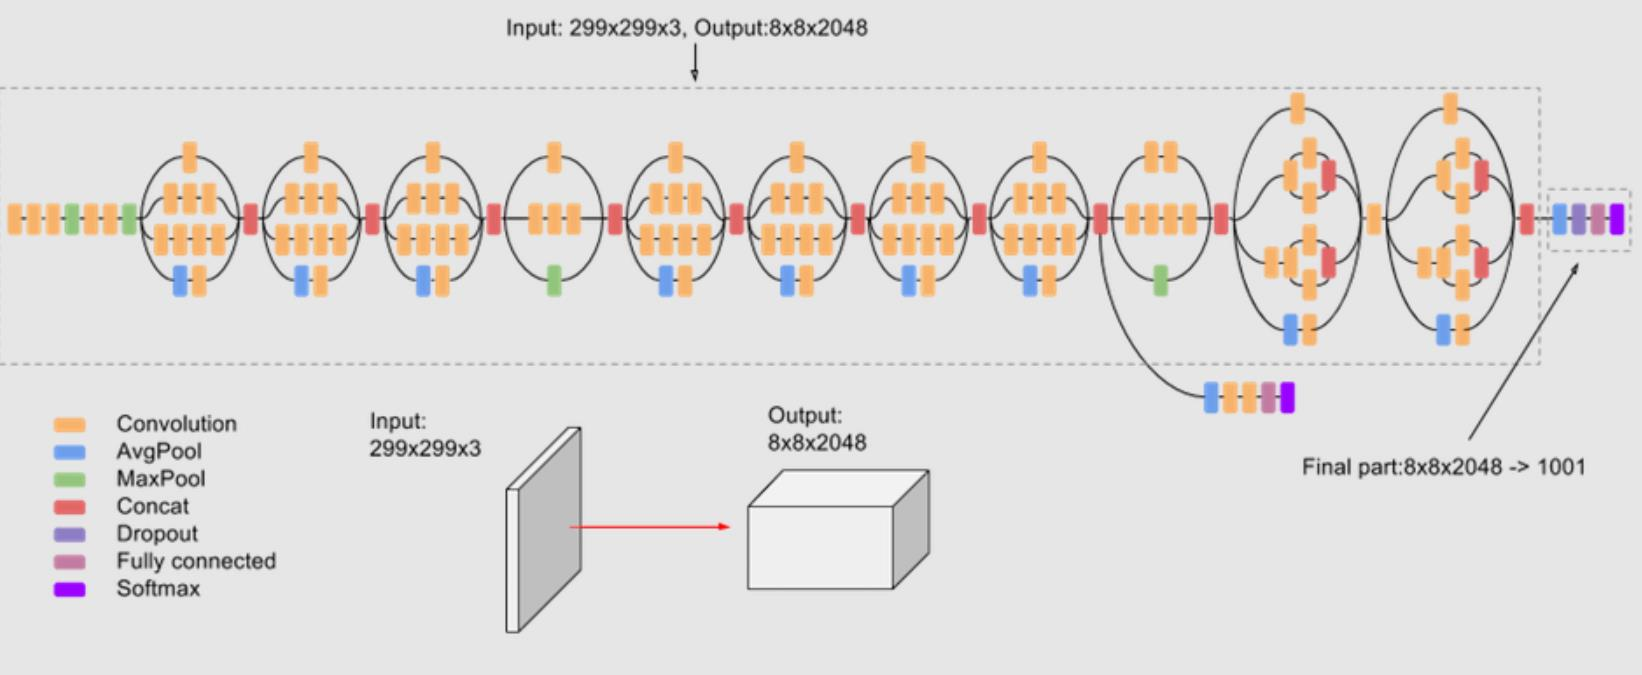
\includegraphics[width=\textwidth]{images/1_inception_v3}
        \caption{Inception V3 Structure}\label{fig:inception-v3}
    \end{figure}
    \item ResNet is a model that is based on the concept of \emph{residual network} which is composed by several blocks of the same type with the skip connections:
    \begin{figure}[H]
        \centering
        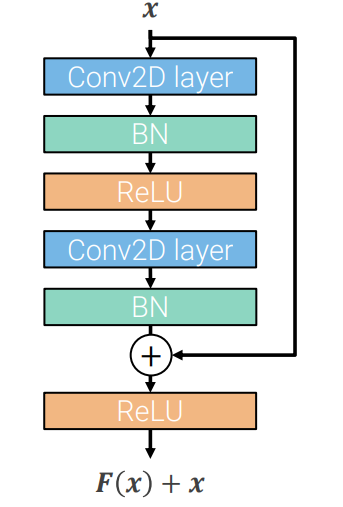
\includegraphics[width=0.4\textwidth]{images/1_1_skip_connection}
        \caption{Skip connection}\label{fig:skip-connection}
    \end{figure}
    Basically, the input of the block is added to the output before feeding it to the next block, in this way, we can avoid the \gls{vanishing gradient problem} making easier the training process.
\end{itemize}
After this, the computer-visionists lend the Transformer architecture (Vaswani et al.~\cite{transformer_paper} from \gls{nlp}, bringing up ViT (Dosovitskiy et al.~\cite{vit_paper}) which is based on the \gls{mha} mechanism.
A multi-head attention is a module for attention mechanisms which runs through an attention mechanism several times in parallel.
In this way, the model can attend to the different parts of the input, forming, in this way, the cross-attention over different parts of the input.

\section{Problem}\label{sec:problem}
The term "odometry" originated from two Greek works \emph{hodos} (meaning "journery" or "travel") and \emph{metron} (meaning "measure").
This derivation is related to the estimation of the change in a robot's pose (translation and rotation) over time.
Mobile robot use data from motion sensor to estimate their position relative to their initial location, this is called odometry.
VO is a technique used to localize a robot by using only a stream of images acquired from a single or multiple camera.
There are different ways to classify the typology of Visual Odometry:
\begin{itemize}
    \item based on the camera setup:
        \begin{itemize}
            \item Monocular VO: using only one camera;
            \item Stereo VO: using two cameras;
        \end{itemize}
    \item based on the information:
        \begin{itemize}
            \item Feature based method: which extracts the image feature points and tracks them in the image sequence;
            \item Direct method: a novel method which uses the pixel intensity in the image sequence directly as visual input.
            \item Hybrid method: which combines the two methods.
        \end{itemize}
    \item Visual inertial odometry: if a \gls{imu} is used within the VO system, it is commonly referred to as Visual inertial odometry.
\end{itemize}
We can represent the pose in different ways, for example: \textbf{euler angles}, \textbf{quaternions}, \textbf{rotation matrices} combined with \textbf{translation vectors}.

The goal is to create a \gls{nn}, using a \textbf{ResNet} to extract features from images and the \textbf{transformer} presented by ~\cite{transformer_paper}, which is able to estimate a sequence of camera poses1. given a sequence of images.
%! Author = wxw85
%! Date = 01/08/2022

\section{Solution}\label{sec:solution}
%**************************************************************
To solve the problem of visual odometry, we tried different approaches to feed the data into the model, and to construct the model itself.
We tried following approaches to feed the data:
\begin{itemize}
    \item Feeding the sequence into the model directly and presenting the pose as \emph{euler angles}.
    \item Feeding the sequence into the model directly and presenting the pose as \emph{rotation matrix} so with twelve numbers and \emph{translation vector}.
    \item Feeding the sequence into the model where the first frame is the origin of the reference frame and presenting the pose as \emph{euler angles}.
    \item Feeding the sequence into the model where the first frame is the origin of the reference frame and presenting the pose as \emph{rotation matrix} and \emph{translation vector}.
    \item Feeding the sequence into the model where the first frame is the origin of the reference frame, and using the auto-regressive model to predict the pose.
\end{itemize}

We used these input strategies to feed the sequence, we tried different variants of models:
\begin{itemize}
    \item Using the different version of ResNet (producing \gls{embedding} of size 512 and 2048) model as feature extractor attached to the transformer with only encoder part.
    \item Using a \gls{mlp} for the images divided into patches to extract the features, and concatenating all the features as a single embedding then feed it into the only-encoder version of transformer.
    \item Using a MLP for the images divided into patches to extract the features, and concatenating all the features as a single embedding then feed it into the encoder-decoder version of transformer.
    \item Using the different version of ResNet model as feature extractor attached to the transformer with encoder and decoder.
    \item The same model as the previous but implemented in \gls{auto-regressive} mode.
\end{itemize}
\section{Results}\label{sec:results}

% %**************************************************************

\subsection{Full sequence prediction}\label{subsec:full-sequence-prediction}
With different models a variety of results are achieved, but the most important result is that an important baseline for the future development of this kind of systems has been settled down.
After a few trials with few models, which produced some circular trajectories, with the encoder-only version of transformer, and feeding the \textit{sequence 3} of Kitti (for more details \S~\ref{sec:kitti}) where the first image is considered as origin, we showed that the model is able to learn a single sequence in over-fitting, but fails when trying to over-fit a more complex sequence.

The encoder-decoder version achieved the same results as the previous version, but the model was able to learn also the \textit{sequence 7} of Kitti, but it fails when trained with both \textit{sequence 3} and \textit{sequence 7}.
\begin{figure}[H]
    \centering
    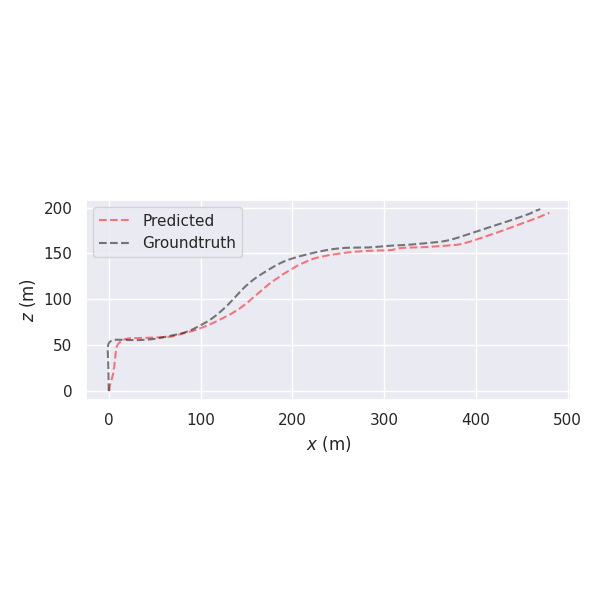
\includegraphics[width=0.8\textwidth]{images/1_4_well_predicted_seq_3}
    \caption{Good prediction sequence 3}\label{fig:well-predicted-seq-3}
\end{figure}
\begin{figure}[H]
    \centering
    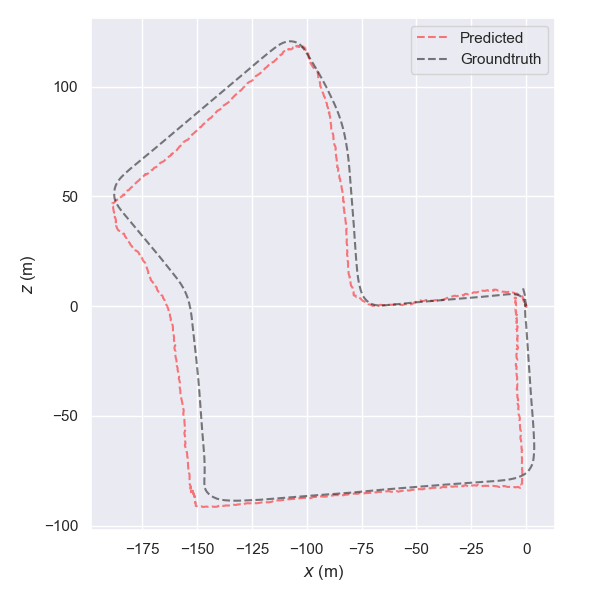
\includegraphics[width=0.8\textwidth]{images/1_4_well_predicted_seq_7}
    \caption{Good prediction sequence 7}\label{fig:well-predicted-seq-7}
\end{figure}
% %**************************************************************

\subsection{Autoregressive models}\label{subsec:autoregressive-model}
We implemented only the encoder-decoder version of the transformer in the autoregressive way, and most of the time the prediction of the network during the training on seq 3 is just a straight line.
So the model is \textbf{not} able to predict the simplest sequence in over-fitting.
The model could not predict any reasonable trajectory, predicting only a linear trajectory as the follow:
\begin{figure}[H]
    \centering
    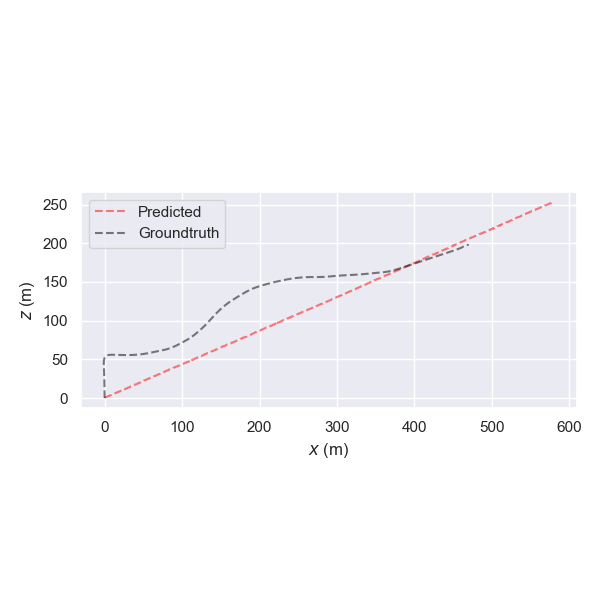
\includegraphics[width=0.8\textwidth]{images/1_4_autoregressive_prediction}
    \caption{Bad prediction sequence 3 of autoregressive model}\label{fig:autoregressive-seq-3}
\end{figure}
Although the model has been trained for more than two hundred epochs, the network cannot understand the goal, and this maybe is due to the loss function.
\section{Thesis Organization}\label{sec:thesis-organization}
\begin{description}
    \item[{\hyperref[ch:introduction]{First chapter}}] introduces the general content about thesis and gives a short presentation of the topic, the problem and the solution we propose;

    \item[{\hyperref[ch:theoretical-foundations]{Second chapter}}] a deepening about the theoretical foundations used during the stage and the project;

    \item[{\hyperref[ch:datasets]{Third chapter}}] presents the datasets used during for the training and the testing of the model;

    \item[{\hyperref[ch:experiments]{Fourth chapter}}] presents the experiments did during to develop the system;

    \item[{\hyperref[ch:implementations]{Fifth chapter}}] presents the different implementations of the system;

    \item[{\hyperref[ch:final-discussions]{Sixth chapter}}] discusses about the results and possible future developments.
\end{description}
During the drafting of the essay, following typography conventions are considered:
\begin{itemize}
    \item the acronyms, abbreviations, ambiguous terms or terms not in common use are defined in the glossary, in the end of the present document;
    \item the first occurrences of the terms in the glossary are highlighted like this: \gls{word};
    \item the terms from the foreign language or jargon are highlighted like this: \emph{italics}.
\end{itemize}
